
\documentclass[a4paper,12pt,oneside]{article}

%%%% PACKAGES %%%%

\usepackage[T1]{fontenc}
\usepackage[utf8]{inputenc}
\usepackage{fourier}
\usepackage[danish]{babel}
\usepackage[danish]{cleveref}
\usepackage{graphicx}
\graphicspath{{Images/}}
\usepackage{pdfpages}
\usepackage{csquotes}

\title{Procesanalyse}
\author{\textbf{SW2-A405a} \\ \\
Simon Vandel Sillesen\\
Kasper Kohsel Terndrup\\
Alexader Krog\\
Mikkel Lægteskov Sø Madsen\\
Frederik Højholt Andersen}
\date{21. maj 2014}

\begin{document}
\maketitle

\section{Indledning}

I denne procesanalyse beskriver og reflekterer gruppen over hvilke teknikker og metoder der blev brugt i 2. semesterprojektet omkring bådudlejning.  I slutningen af analysen, beskrives hvilke elementer af gruppearbejdet der skal fortsættes med og hvilke der skal stoppes.

\section{Beskrivelse}

Her vil komme en beskrivelse af vores arbejdsprocesser i P2. Det er en objektiv beskrivelse af hvad der skete og hvad vi gjorde.

\subsection{Projektplanlægning}

Trello blev brugt til at holde styr på hvilke opgaver der skal laves. Trello er en gratis webbaseret projektledelse værktøj (bilag 1). På Trello blev der lavet en virtuel opslagstavle til projektet. En opslagstavle indeholder lister, som hver består af kort som svarer til en opgave. Man kan flytte opgaverne via. drag \& drop. Der blev lavet 3 lister: TODO som bruges til opgave der skal laves, DOING som man kan flytte opgaverne hen på, når man starter med at lave dem, og DONE som man flytter opgaverne hen på når man er færdig. På Trello blev der derudover også lavet en liste med milepæle. Hver milepæl fik tildelt en dato, hvor den skulle være færdig. Ud over listen af milepæle var der ikke lave nogen anden tidsplan

Der var ikke udpeget en projektleder, så alle i gruppen var ligestillet. Der var ingen der havde specifikke opgaver eller ansvarsområder. Arbejdsopgaverne blev fordelt efter fri vilje. På Trello kunne man "sætte" sig på en opgave, hvis man gerne vil lave den. Der var nogle opgaver der blev hængende i lang tid, fordi der ikke var nogen der ville lave dem.

Kontakt udadtil, det vil sige til Vestre Baadelaug, gik gennem mail og telefon, og opmøde på deres havn. Der blev delt viden omkring havnene i Aalborg med andre grupper på semesteret.

\subsection{Problemformuleringer}

Det var problemer ved at finde en god problemformulering, da vi havde svært ved at finde et problem, der passede til vores oprindelige vinkel. Problemanalysen gjorde det klart, at udgangspunktet for projektforslaget, var svært at finde i en lokal kontekst i Aalborg. Der blev lavet mange iterationer af problemformuleringen, som blev sendt til vejleder, og kom tilbage med respons. Der blev skrevet et refleksionsafsnit, som havde en stor andel, i begrundelsen for problemformuleringen. Vi endte med at fokusere på en push strategi, hvor producenten påpeger et latent behov hos kunden, i modsætning til den mere traditionelle pull strategi, hvor producenten opfylder et aktivt behov hos kunden.

\subsection{Rapportstrukturering}
Rapporten er delt op i to store dele, analysen og løsningen. Analysen omhandler forhold hos dem vi vil designe programmet til. Analysens struktur er baseret af Laudon \& Laudon modellens hovedpunkter som mennesker, teknologi og organisation.

Løsningen bruger det vi fandt ud af i analysen, og designer og implementerer en passende løsning til problemstillingerne fundet i analysen. Først var løsningen opdelt efter emne, men dette blev senere ændret, således at løsningen blev opdelt i et teoretisk afsnit, et implementationsafsnit og et afsnit om aftestning af programmet.

Udover analysen og løsningen består rapporten af et diskussionsafsnit, perspektiveringsafsnit og en konklusion.

For at opretholde en rød tråd, var rapporten igennem flere iterationer. Disse iterationer bestod i at sørge for at sammenhængen mellem analysen og løsningen var overensstemmende. Dette blev gjort ved at gennemlæse rapporten af alle gruppens medlemmer.

\subsection{Gruppesamarbejde}

Vi startede gruppesamarbejdet med at snakke om vores forventninger og erfaringer. Vi har et højt ambitionsniveau i gruppen og det afspejles blandt andet i mødetider, vejleder møderne, strukturen, motivationen i gruppen samt samarbejdsaftalen som kan findes i bilag 2. Gruppens medlemmer havde forskellige forudsætninger, forud for gruppedannelse, nævneværdigt ét medlem som havde skiftet til Software, fra et andet studie. Vi valgte at lave en samarbejdsaftale så vi havde et reglement for gruppens velvære og samarbejde. Samarbejdsaftalen er udarbejdet mundtligt og derefter skrevet ned og godkendt af alle gruppens medlemmer.

Vi holdte møder næsten dagligt omkring status, omkring hvor langt gruppens medlemmer er kommet med deres opgaver og om der evt. er noget der skal vendes med gruppen. Disse forekom på forskellige tidspunkter når det føltes rigtigt at have et. For eksempel efter frokost hvis gruppen blev useriøs og vi havde brug for at komme tilbage på sporet. Møderne har været åbne for alt, så der blev snakket om alt fra fridage, hvad vi skal efter fyraften, til hvad planen for projektet er lige nu og evt. hjælp med opgaver i andre kurser. Hvis et gruppemedlem ikke er tilstede til mødet fortsættes der uden vedkommende, men der blev ofte taget et statusmøde dagen efter for at få medlemmet tilbage på sporet hvis der blev diskuteret noget vigtigt. Derudover blev der ofte benyttet \enquote{Skype} til at kontakte det manglende medlem og holde medlemmet up to date. Gruppen har haft fast mødetid fra 08:15-16:15 og disse er blevet overholdt. Dog i situationer hvor medlemmer arbejder hjemmefra, er \enquote{Skype} også benyttet her.

I gruppen har vi haft en åben og seriøs tone, som har hjulpet med at man kan give og modtage kritik, uden at tage det personligt. Derudover har vi også haft mange diskussioner som ofte endte med at trække ud.

Gruppen har nogle medlemmer der snakker meget, og andre medlemmer der ikke snakker så meget. Dog har de medlemmer der snakker meget en god disciplin, og lader dem der ikke snakker så meget få lov til at tale.

Der har været svingende/manglende motivation hos nogle medlemmer. Men dette blev afviklet med en sund og konstruktiv samtale med medlemmerne, med fokus på trivsel i gruppen og årsagen til den svingende eller manglende motivation.

Gruppen har uddelegeret opgaverne efter et frit-for-alle princip. Dvs. gruppens medlemmer selv skulle tage initiativ og melde sig på opgaverne. Dog har der været fokus på at alle skal prøve at arbejde på alle områder, så vi ikke ville ende med medlemmer der kun havde viden omkring deres arbejdsområde. Dog er der uddelt arbejdsområder til medlemmer med unik ekspertise for området.

Vi har i gruppen haft en professionel og positiv tilgang til kritik. Hver gang et afsnit eller modul i programmet er blevet lavet, er det blevet vendt i gruppen og der er et gruppemedlem der har gået det igennem med medlemmet der har lavet det. Derudover har vi løbende læst afsnit igennem for at sikre alle ved hvad der skal laves. Udover dette har vi også sat \enquote{Fix Me’s} i rapporten med relevante tekster, som har fungeret som milepæle for gruppen. \enquote{Fix Me’s} er arbejdsnoter, rettet imod gruppen selv.

\subsection{Samarbejde med vejleder}
Kontakten til vejlederen Brian Nielsen foregik gennem en mailkorrespondance, samt ugentlige vejledermøder. Tidspunkter for vejledermøderne blev oftest aftalt på det foregående vejledermøde, og blev for det meste afholdt mandag morgen. Mandag var den ene dag om ugen hvor på gruppen ikke havde nogen planlagte kurser. 

Der blev udarbejdet en samarbejdsaftale af gruppen som herefter blev godkendt af vejlederen, kan se på bilag 3. 

Forud for samtlige vejledermøder blev der udarbejdet et skriftligt arbejdsblad, samt læsevejledning, som blev tilsendt vejlederen. Under møderne blev et af gruppens medlemmer udnævnt som referent for vejledermødet. Korte spørgsmål blev sent og besvaret per mail.

Der blev ikke sendt kodeeksempler til vejlederen, men udelukkende rapport.

\subsection{Programmering}

Programmering blev først påbegyndt kort efter statusseminaret. Alle i gruppen fulgte med på projektor, da vi lavede den første udgave af modelleringen af havnen. Under den grundlæggende programmering, arbejdede vi primært i hold af to, hvor vi skiftede én af de to ud, således at der hele tiden var en "erfaren" og en "ny". Microsofts Visual Studio blev anvendt til de strukturelle områder, og blev brugt som editor af alle. Der var en løs aftale, om at anvende TODO's i C\#. Der blev oprettet TODO's, men få blev løst. Git blev anvendt til at synkronisere filer, og til versionskontrol. Test Driven Development blev planlagt, men ikke gennemført til fulde. Senere i forløbet blev programmet omformet, til en mere modulær opbygning.

\section{Vurdering og Analyse}

Her vil vi vurdere hvordan projektet gik, og prøve at analysere hvorfor det gik sådan. 

\subsection{Projektplanlægning}

Gruppen vurderer projektplanlægningen som god, på trods at den lave mængde tidsplanlægning. Gruppen føler ikke at tidsplanlægning har manglet, eller at yderligere tidsplanlægning ville bidrage til et bedre projekt. De daglige statusmøder holdte fokus, og var gode til at sikre én fælles retning af rapporten. \enquote{Trello} hjalp meget, især med at holde styr på de mindre detaljer i større opgaver. På dage hvor der blev samlet løse ender, var \enquote{Trello} også godt til at tildele sig selv opgaver, uden at skulle forstyrre gruppen. \enquote{Fix me}s i rapporten har også været en enorm hjælp når et afsnit skulle viderebehandles af et andet gruppemedlem. Planlægning med vejleder gik flydende, da begge parter var glade for mandag morgen som mødetidspunkt. Det gav også gruppen en fin rytme. Kontakt udadtil var god, især grundet et hjælpsomt baadelaug. Vidensdeling med andre grupper, fungerede godt, på trods af enkelte uenigheder omkring prioriteter.

\subsection{Problemformuleringer}
Problemformuleringen endte med at blive god. Det skete efter et godt samarbejde med vejlederen. Vi havde problemer i starten, fordi vi gik for meget efter at finde et problem. Men i Vestre Baadelaug var det svært at finde et problem. Det gjorde os lidt bange, da vi troede alt vores arbejde var spildt, da de ikke havde nogle problemer. Men det var godt at Brian ledte os på sporet og fik os til at se efter muligheder ved implementation af et it-system.

Det var også godt med et statusseminar hvor man fik chancen for at fremlægge sin problemformulering og få feedback på den, fra nogen udefrakommende. Vejleders feedback var også godt til at få lavet små ændring til problemformuleringen, hvis der var noget der var utydeligt.

\subsection{Rapportstrukturering}

Det var godt vi delte rapporten op i en analysedel og en løsningsdel, fordi det så var nemmere først at arbejde med analysen, og senere designe en løsning, når vi havde tilstrækkelig information omkring den ønskede løsning.

Laudon \& Laudon modellen var god til at skabe en skabelon til de emner, der er vigtige at beskrive i en analyse. På den måde fik vi ikke beskrevet unødige emner, som ingen relevans havde for projektet. Det var også nemmere at gå i gang med analysen, fordi vi vidste hvad store dele af analysen skulle omhandle.

Strukturen af rapporten blev god, da at vi lavede en hård opdeling af det teoretiske afsnit i løsningen og implementationsafsnittet i løsningen. Herved blev det nemmere at skabe en rød tråd igennem løsningen i rapporten, og der blev undgået at beskrive en implementation af en teori, der endnu ikke var beskrevet tidligere i rapporten.

\subsection{Gruppesamarbejde}

Samarbejdsaftalen fungerede godt for gruppen. Dog blev den aldrig hevet frem i diskussioner, men den gjorde at gruppen fik et reglement og ordentlig struktur. Uddelegeringen af opgaver har fungeret godt for gruppen, og alle medlemmer ved meget om alle aspekter af programmet og rapporten, dog er der stadig eksperter på specielle områder. Igennem forløbet prioriterede vi vidensdeling højt, og sørger for at alle i gruppen havde forståelse af alt fra status til opgaver. Til dette brugte vi vores statusmøder hvor vi kunne snakke omkring alt. Møderne virkede rigtig godt, og de gav en følelse af åbenhed i gruppen. Det hændte at der blev holdt status på baggrund af tvivl omkring hvilket arbejde der skulle udføres, hvorefter det blev afklaret og gruppen kunne arbejde videre. Dette synes vi er et stort plus, da man ellers ville sidde inde med det. Gruppen ligger stor vægt på at have et velkommende arbejdsmiljø hvor man trives og ser frem til at komme til.

Vi har brugt Facebook til at kommunikere korte beskeder frem og tilbage. Dette var alt fra meldinger af sygdom til invitation til events. Vi brugte Github til at synkronisere vores arbejde, og let flette ændringer sammen. Dette hjalp også med at give et overblik over hvilke ændringer der er blevet lavet. Github gjorde at vi kunne kigge nærmere på ændringerne og få en øget forståelse af projektets helhed. 

Rapporten er skrevet i LaTeX hvilket har givet en flot struktur i rapporten. Dog er der nogle medlemmer der havde begrænset kendskab til programmet der havde svært ved at benytte programmet. Trods dette lærte medlemmerne hurtigt at benytte programmet. Ofte diskuterede vi i gruppen, og diskussionerne omkring vigtige beslutninger for programmet og rapporten har ofte trukket langt ud. Dog synes vi at udbyttet og grundigheden af diskussionen har været tiden værd, siden diskussionspartner går fra diskussionen med et nyt syn på emnet.


\subsection{Samarbejde med vejleder}

Gruppen har været tilfreds med vejledersamarbejdet. Der har været en passende mængde interesse fra vejlederens side, og vejledere var god til at pointere områder, hvor gruppen burde øge fokus. Antallet af møder, passede gruppen godt. Frekvensen var høj nok til at nyt arbejde var klart, til at blive taget op på møderne, men også tæt nok, til at gruppen oplevede et positivt pres, med ugentlige deadlines.

Gruppen oplevede enkelte misforståelser under kommunikation med vejlederen, som skabte lidt forvirring omkring det ønskede resultat. Det vurderes dog til at være grundet i uklare udmeldinger fra gruppens side, samt manglende indspørgen til specifikke ting.

Gruppen ville også gerne have delt kodeeksempler med vejlederen, da det muligvis kunne have givet vejlederen en bedre forståelse for visse dele af rapporten.

\subsection{Programmering} 

I gruppen mener vi selv at slutproduktet blev en succes, men med store problemer undervejs grundet en mindre misforståelser i gruppen omkring modellering af havnen. Vi lagde ud med at modellere havnen i fællesskab inden programmerings processen blev påbegyndt, hvilket vi har været godt tilfreds med. Vi mener derimod også at vi burde have lavet flere revurderinger af programmet løbende.

Vores udgangspunkt var at benytte test driven development, men fandt det svært at skrive test til visse dele af programmet heriblandt database. Derfor valgte vi at skrive programmet færdigt uden brug af test driven development. Programmet inddelte vi i moduler for at gøre det nemmere for gruppen af uddelegere arbejdsopgaverne. Vi mener at vidensfordeling omkring programmet har været godt, samt at alle fra gruppen har arbejdet med alle dele af programmet. 

Gruppens plan om at benytte os af visual studio's TODO funktion fungerede ikke grunde der ikke blev snakket om hvordan det skulle bruges. Koden blev ikke dokumenteret grundet tidspres og manglede kommunikation blandt gruppen medlemmer omkring hvordan koden skulle dokumenteres. Vi mener at det burde været prioriteret højere.


\section{Bilag} 
\label{sec:bilag}

Herunder følger bilag til procesanalysen. Ethvert bilag fylder én side.

% section bilag (end)

\includepdf[pages={1}]{trello.pdf}
\label{trello}
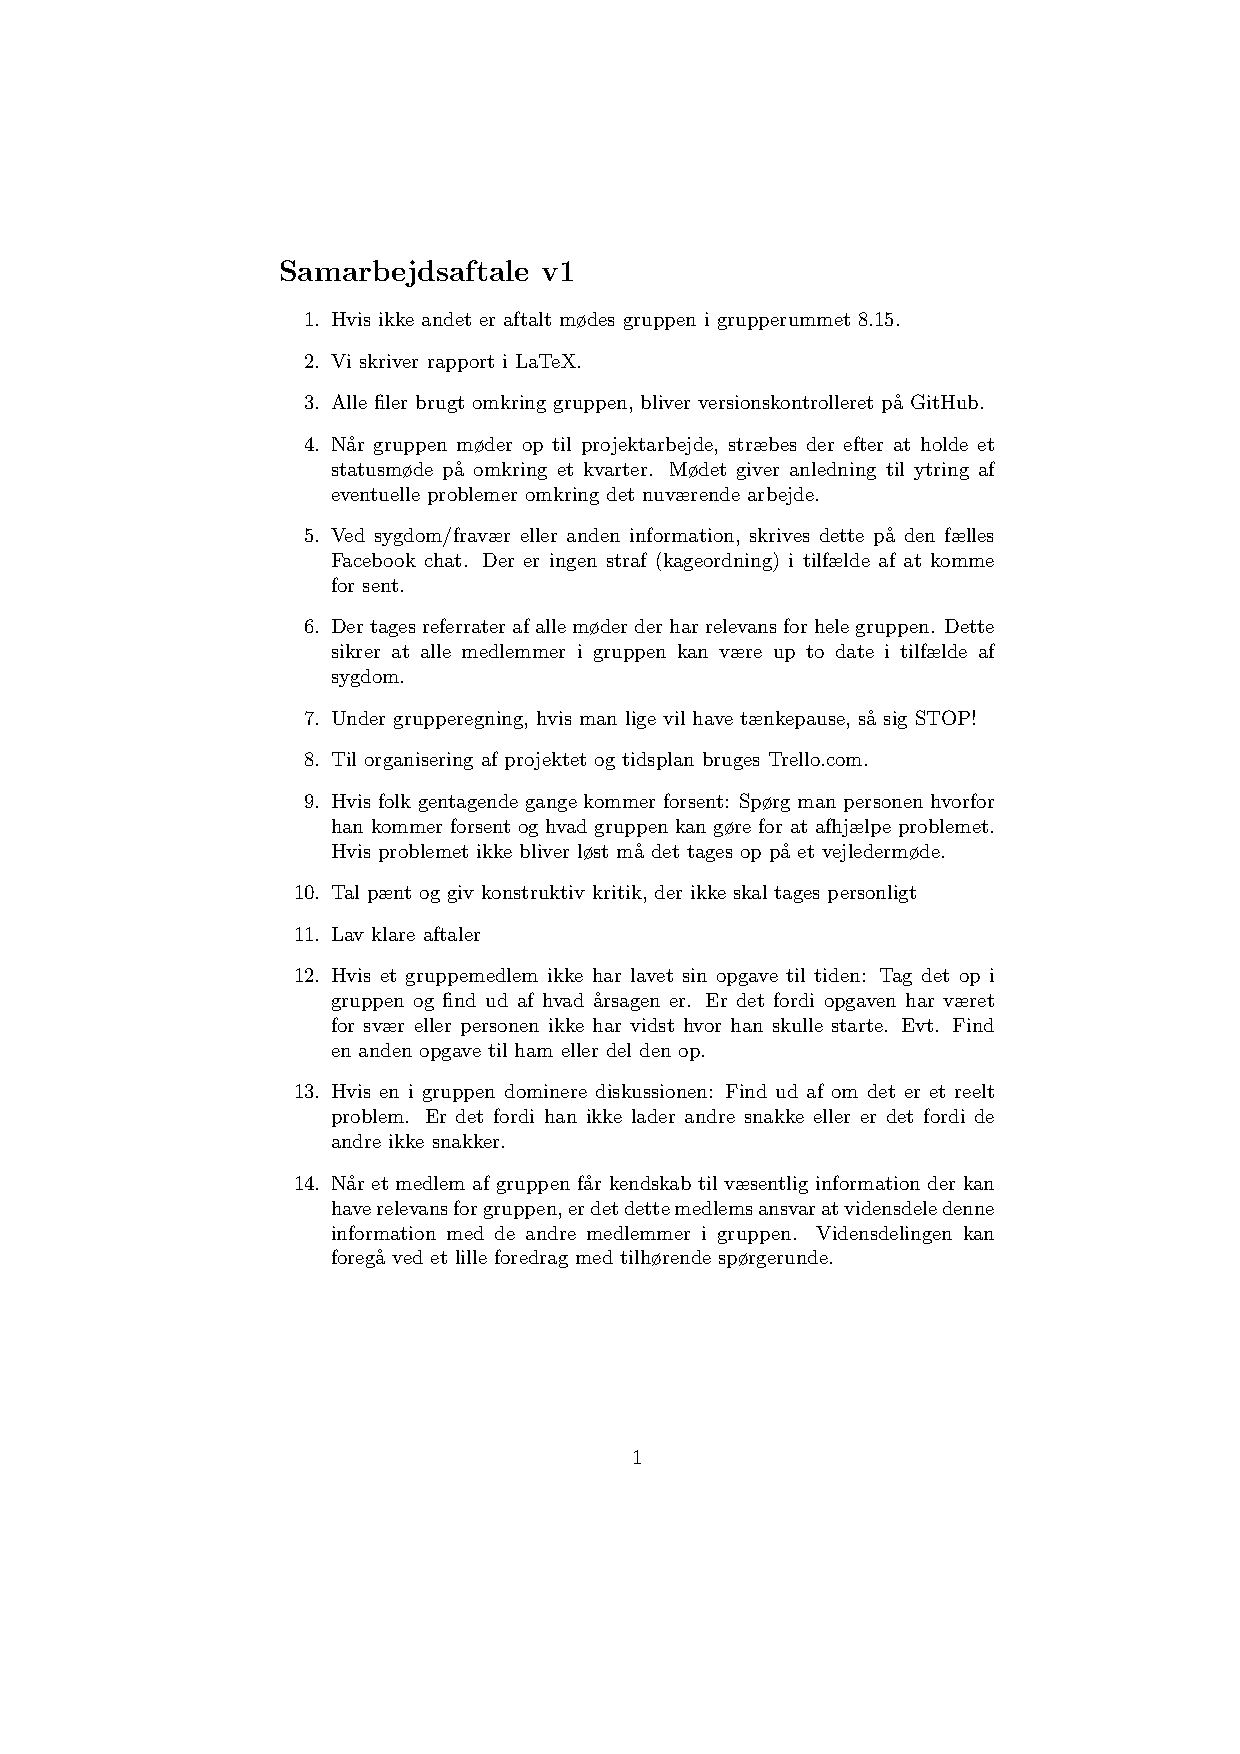
\includepdf[pages={1}]{samarbejdsaftale.pdf}
\label{samarbejdsaftale}
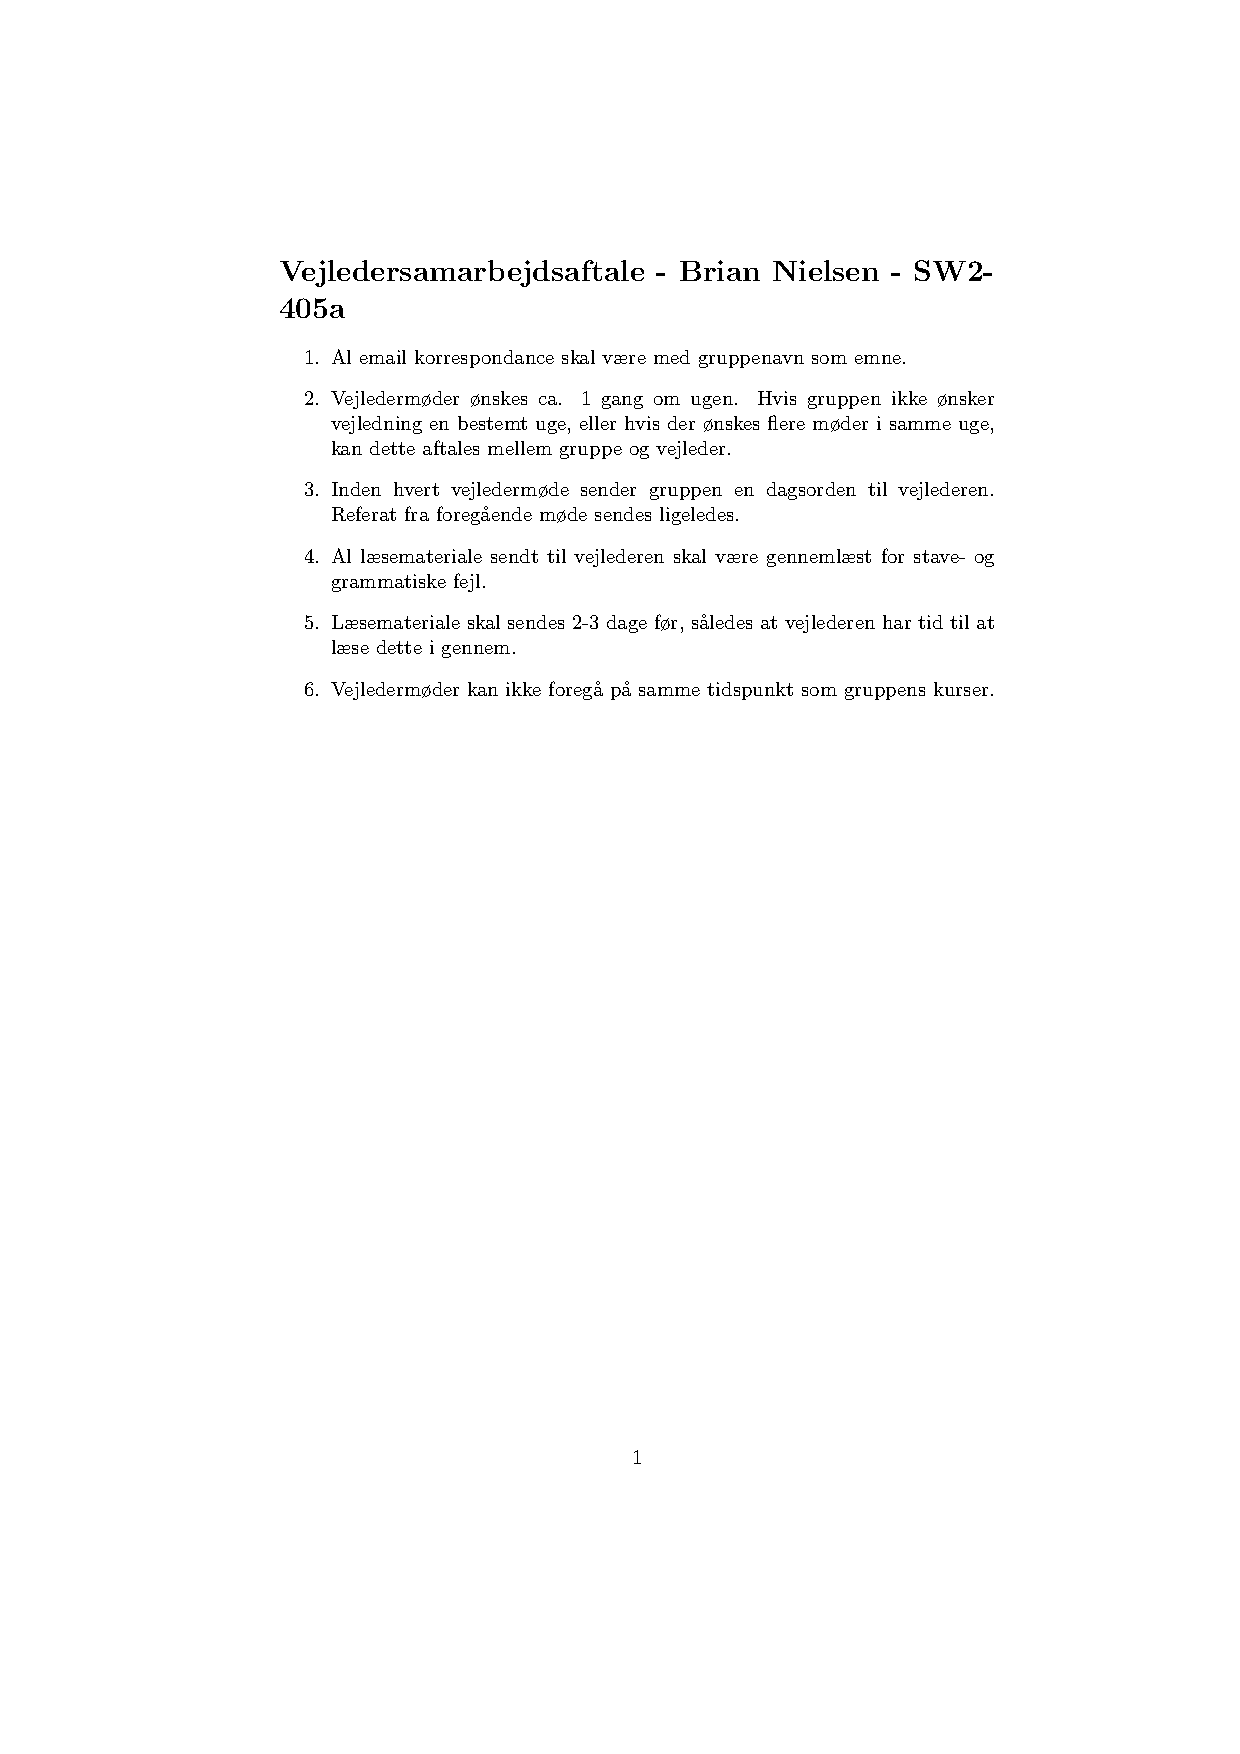
\includepdf[pages={1}]{vejleder-samarbejde.pdf}
\label{vejledersamarbejde}
\end{document}
